\documentclass[10pt,a4paper,final]{scrartcl}
\usepackage[utf8]{inputenc}
\usepackage{amsmath}
\usepackage{amsfonts}
\usepackage{amssymb}
\usepackage{graphicx}
\usepackage{float}
\author{
Group No.: 05 \\ 
Group Members: \\
LIU Xinhong (53043714) \\
LI Tong (53043505) \\
ZHONG Yuqing (53057522)
}
\titlehead{
City University of Hong Kong \\
Department of Electronic Engineering
}
\title{
EE3316 Information Product Design \\ Mobile App Design Final Report \\ 2013/14 (Semester B)}
\subtitle{Into Heart}
\begin{document}
\maketitle

\pagebreak

\begin{abstract}
Heart is a vital organ of human body, once it stops, no matter how strong, you are gone.  
This app monitors heart rate all-day and evaluate heart health condition, integrates into everyday exercise training session and help user to control the exercise strength, to reach a better exercise goal, as well as training heart. With social integration, this app connects user with friends and family to motivate user care about their heart. This app also conducts emergency alert including: contacting the family, call ambulance, make noise, or any other viable first aids. 
\end{abstract}



\tableofcontents

\section{Introduction}

\subsection{Market Research}

Cardiovascular diseases (CVDs) are a group of disorders of the heart and blood vessel. In 2012 it kills 17 million people, makes 31\% of all death in the world\footnote{WHO, Cardiovascular diseases (CVDs), retrieved from http://www.who.int/mediacentre/factsheets/fs317/en/ on Feb 2, 2015 }. 
According to some researches, heart rate (HR) is an independent predictor of cardiovascular and all-cause mortality in men and women with and without diagnosed cardiovascular disease1. Heart rate was assigned the same weighting as blood pressure and cardiorespiratory fitness in the overall score1. On the other hand, It's vital to monitor your heart rate during exercise3. A target heart rate is recommended to reach best exercise goal. Time is important when heart attack suddenly occur, time is life, handling emergency situation is a problem when patient is not near there relatives. 

\subsection{App Summary}
\subsection{Target User Group}
\subsection{Competitive Analysis}

\section{App Design and Analysis}
\subsection{Architectural Design}
\begin{figure}[H]
\centering
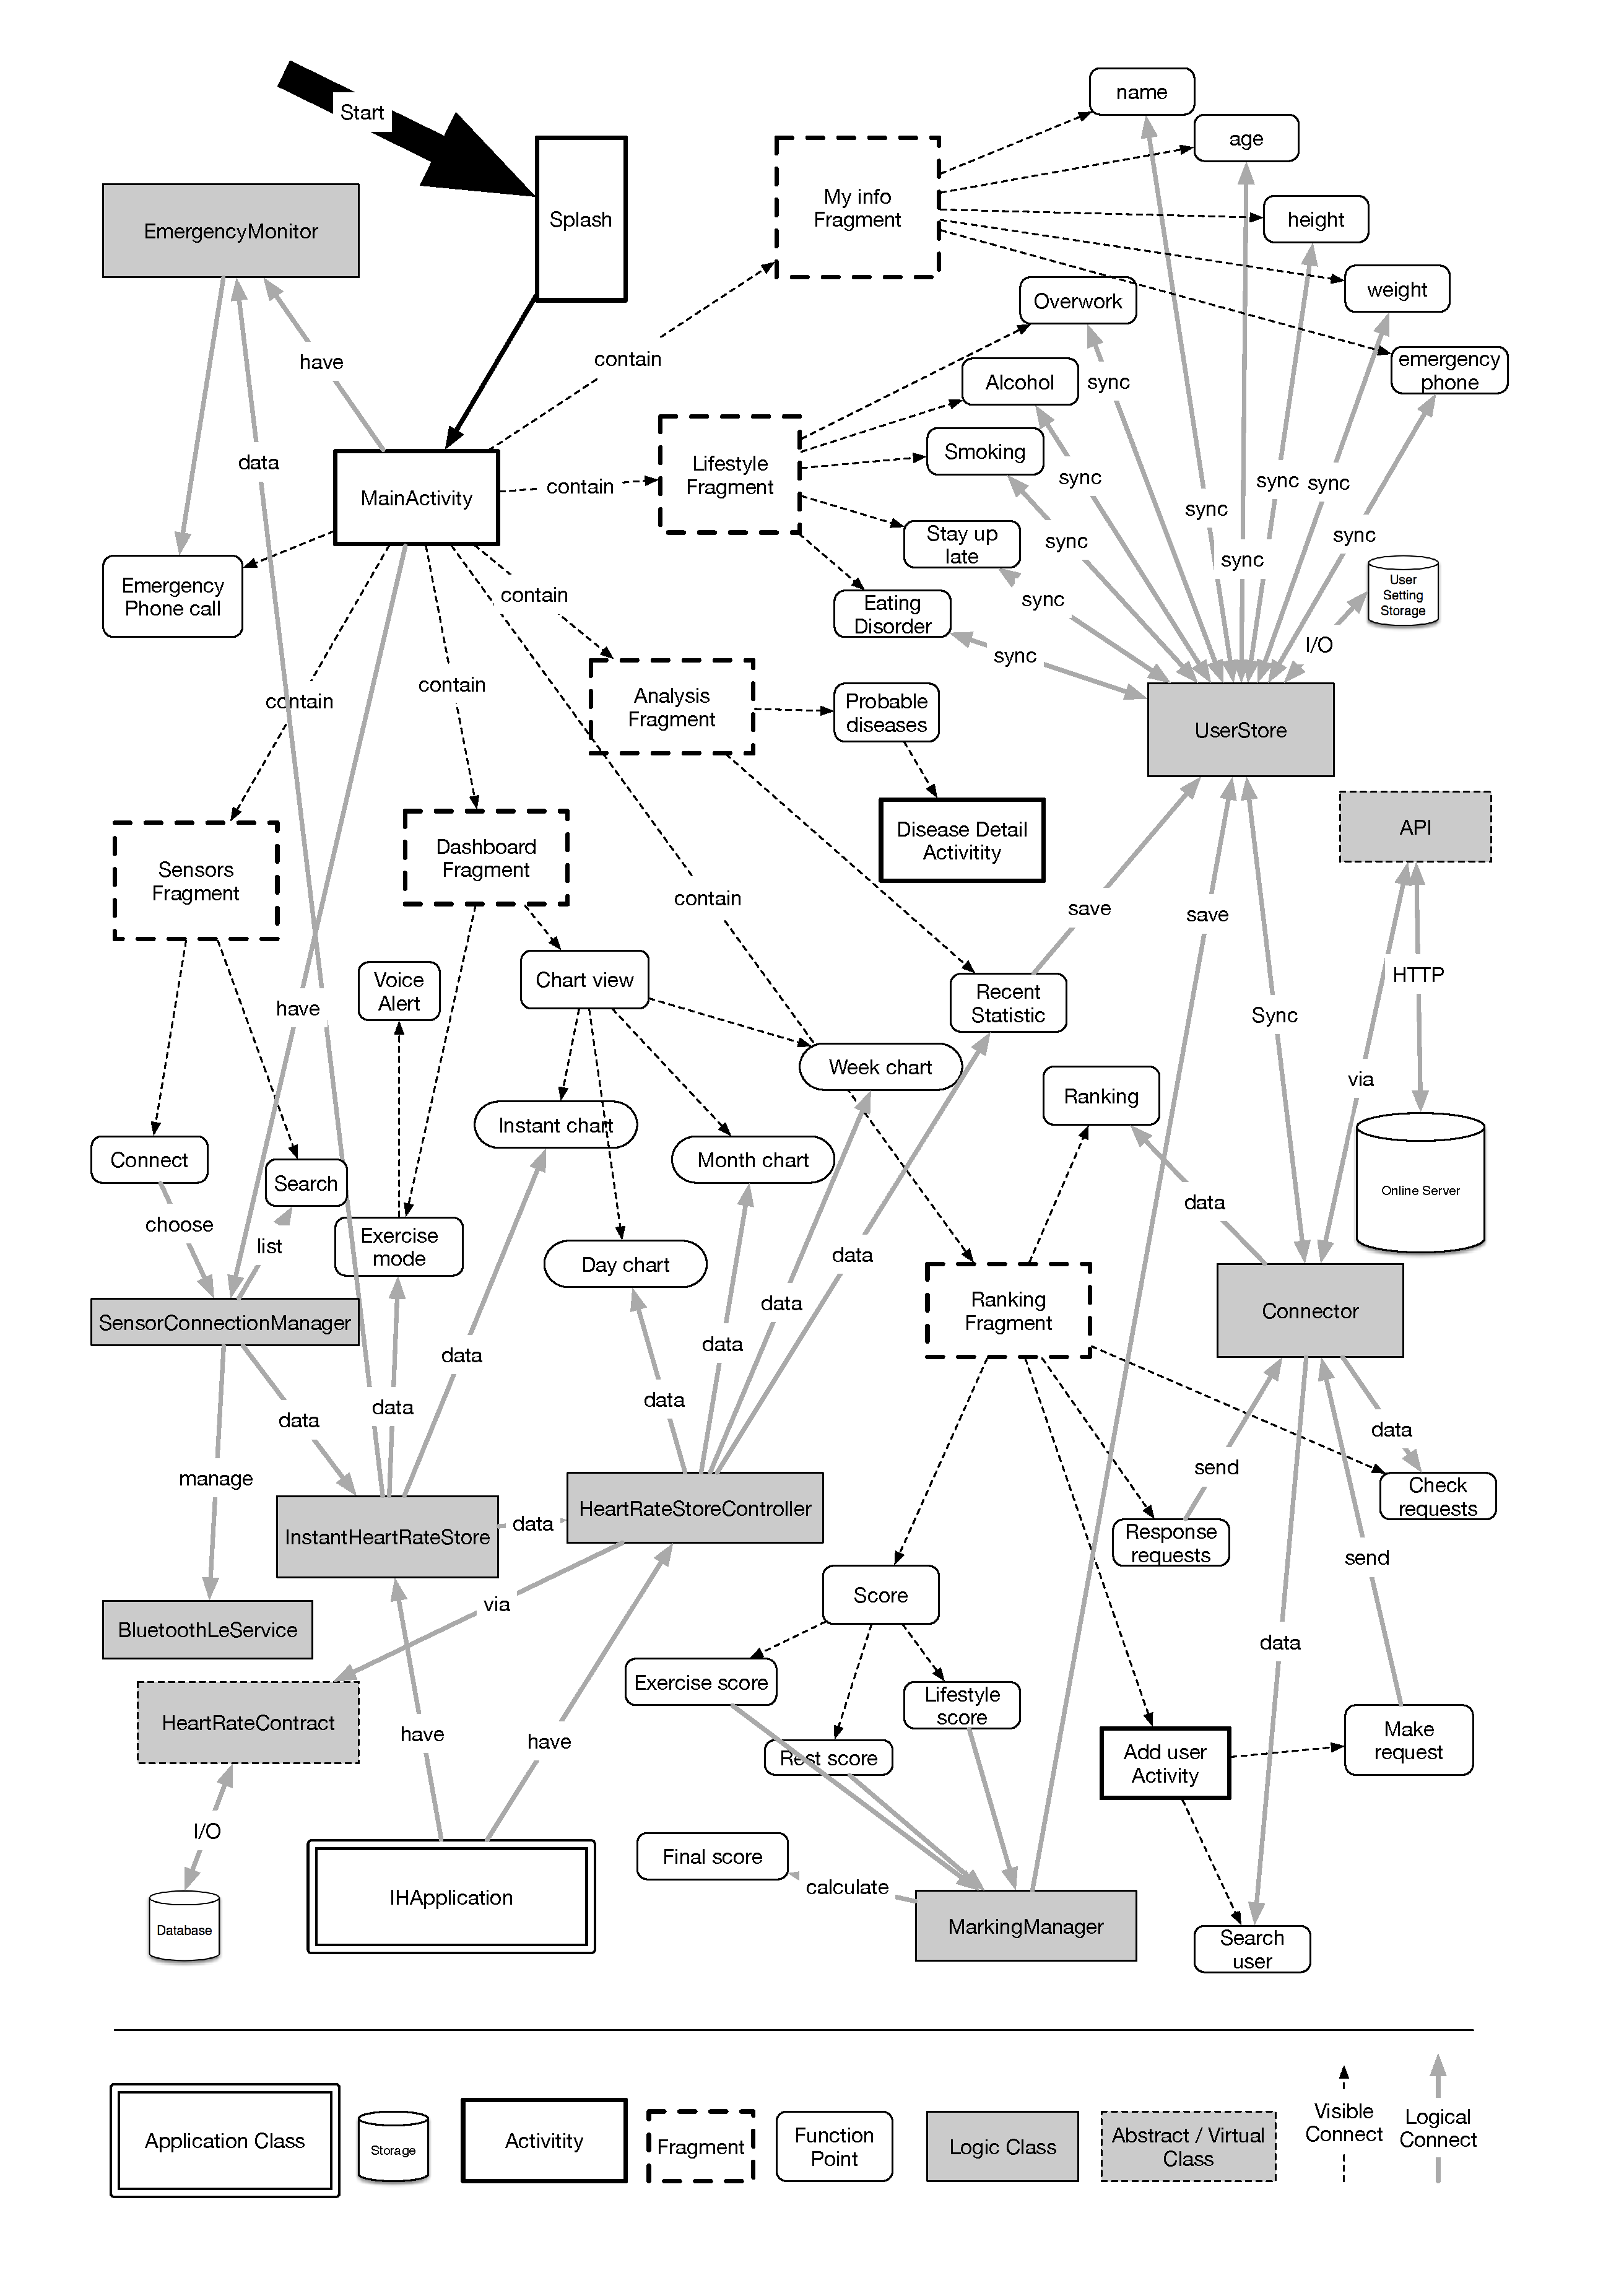
\includegraphics[width=5.3in]{img/arch.eps}
\caption{Into Heart Architectural Design}
\end{figure}

\end{document}